\documentclass[a4paper]{article}

\usepackage[sort]{natbib}
\usepackage{fancyhdr}


% \documentclass[a4paper]{article}

\usepackage[english]{babel}
\usepackage[utf8]{inputenc}
\usepackage{amsmath}
\usepackage{graphicx}
\usepackage[colorinlistoftodos]{todonotes}
\usepackage{hyperref}
\usepackage{booktabs} % To thicken table lines
\usepackage{tablefootnote}
\usepackage{listings}
% \usepackage[numbers]{natbib}

\usepackage{graphicx}
\usepackage{babel,blindtext}

\usepackage{algorithm}
\usepackage[noend]{algpseudocode}


% Uirá packages
\usepackage{algorithm}
\usepackage[noend]{algpseudocode}
\usepackage{booktabs} % To thicken table lines
\usepackage{graphicx}
\usepackage{babel,blindtext}
\usepackage{amsmath}
\usepackage[colorinlistoftodos]{todonotes}
\usepackage{hyperref}
\usepackage{mathtools}
\usepackage{listings}
\usepackage{epstopdf}



% you may include other packages here (next line)
\usepackage{enumitem}



%----- you must not change this -----------------
\oddsidemargin 0.2cm
\topmargin -1.0cm
\textheight 24.0cm
\textwidth 15.25cm
% \parindent=0pt
\parskip 1ex
\renewcommand{\baselinestretch}{1.1}
\pagestyle{fancy}
%----------------------------------------------------



% enter your details here----------------------------------

\lhead{\normalsize \textrm{Continuous Control}}
\chead{}
\rhead{\normalsize October 23, 2018}
\lfoot{\normalsize \textrm{DRLND - Udacity}}
\cfoot{}
\rfoot{Uirá Caiado}
\setlength{\fboxrule}{4pt}\setlength{\fboxsep}{2ex}
\renewcommand{\headrulewidth}{0.4pt}
\renewcommand{\footrulewidth}{0.4pt}


\begin{document}


%----------------your title below -----------------------------

\begin{center}

{\bf \large {Continuous Control With Deep Reinforcement Learning \\ \small Uirá Caiado}}
\end{center}


%---------------- start of document body------------------

% The report clearly describes the learning algorithm, along with the chosen hyperparameters. It also describes the model architectures for any neural networks.

 According to  \cite{Duan:2016ur}, significant progress has been made by combining deep learning with the Reinforcement Learning (RL) framework, obtaining impressive results in a range of environments, from arcade games to 3D locomotion and manipulation tasks. Most of the algorithms developed were designed for tasks with high-dimensional state space and discrete actions. However, in the continuous control domain, where actions are continuous and often high-dimensional, these same models struggle to converge like in the discrete actions environments.
 
 In this project, I trained $20$ identical double-jointed arm agents to maintain their hand at a target location for as many time steps as possible. I used the Unity Machine Learning Agents Toolkit\footnote{Source: \url{https://github.com/Unity-Technologies/ml-agents}} to design, train, and evaluate Deep Reinforcement Learning algorithms. These algorithms combine RL with a class of artificial neural network, known as deep neural network, to generalize its past experiences to new ones. I considered to the tests the algorithms Deep Deterministic Policy Gradient (DDPG) and Proximal Policy Optimization (PPO) algorithms.
 
 The environment used for this project is the Reacher environment, from Unity\footnote{Source: \url{https://bit.ly/2OOkxKo}}. A reward of +0.1 is provided for each step that the agent's hand is in the goal location. The observation space consists of 33 variables corresponding to position, rotation, velocity, and angular velocities of the arm. Each action is a vector with four numbers, corresponding to torque applicable to two joints. Every entry in the action vector should be a number between -1 and 1. To solve the environment, the agents must get an average score of +30 over 100 consecutive episodes, and over all agents.

% describes the model architectures for any neural networks

The algorithms implemented in this project that was able to solve the environment used an actor-critic architecture to deal with the high-dimensional action space. As described by \cite{Lillicrap:2015ww}, the model maintains a parameterized actor function $\mu(s | \theta^{\mu})$ which specifies the current policy by mapping states to a specific action. The critic $Q(s, a; \;\theta)$ is learned using the Bellman equation as in Q-learning and is used to evaluate the actions chosen by the actor. The resulting evaluation is used to compose a baseline (or advantage function) that is then used to train the actor model. 
 
 The parameters $\theta$ from both actor and critic models are learned by neural networks with almost the same architecture. The input to these networks consists of a matrix $33 \times 20$ produced by the environment (the size of the state space times the number of agents) and the first layer is a fully-connected linear layer with $400$ neurons and applies a rectifier nonlinearity. It is followed by a hidden layer also consisting of a fully-connected linear layer with $300$ neurons followed by another rectifier. The output layer of the actor-network consists of a fully-connected linear layer with a vector $4\times1$ as output for each agent. The output layer of the critic network includes of a fully-connected linear layer with a single output for each agent followed by a \textit{tanh} activation function that naturally constrains the values between $[-1, 1]$.


% (1) describes the learning algorithm, along with the chosen hyperparameters
The first algorithm tested was the DDPG model, that was first introduced by \cite{Lillicrap:2015ww} as a modification of the Deterministic Policy Gradient algorithm, proposed by \cite{Silver:wt}. As explained by \cite{lapan2018deep}, It belongs to the A2C family and the role of the actor in this method is to estimate the stochastic policy that returns the probability distribution over the actions. The critic is used to calculate the Q-values of the actions so it can be updated using the Bellman equation to find the approximation of $Q(s, a)$ and minimizing the MSE objective. As explained by \cite{Lillicrap:2015ww}, the actor is updated by applying the chain rule to the expected return obtained by the critic network from the actor parameters. As this method is off-policy, we can use the same tricks used by the DQN model, presented by \cite{mnih2015humanlevel}, as the replay buffer and the use of local/target networks to help stabilize the parameters of both actor and critic.

I used a replay buffer size of $100,000$ experiences, mini-batches of $200$ instances and a $\gamma=0.99$ to discount the rewards. The learning rate of the actor was $0.0001$, to the critic was $0.001$, and the networks were updated every two steps. In the critic optimizer, I also introduced a weight decay of $0.0001$. As suggested by \cite{Lillicrap:2015ww}, the target networks slowly tracked the local networks using $\tau=0.001$. For detail on how each one of these parameters was used in the model, check the papers cited or the code provided along with this report.

Both local and target networks presented the same architecture, described before. Using this configuration, I was able to solve the environment in $309$ episodes. The figure \ref{fig:ddpg} presents the results of the simulation. The left panel exposes the rewards obtained in each episode and, in the right panel, I plotted a moving average of the last $100$ episodes of this rewards. The shaded area corresponds to one standard deviation $\sigma$ of the rewards of those $100$ episodes.

\begin{figure}[ht]
\centering
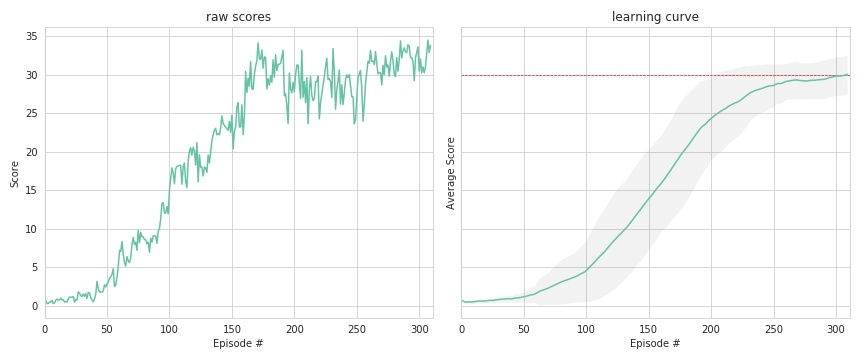
\includegraphics[width=0.65\textwidth]{../notebooks/figures/2018-10-07-DDPG-learning-curve.jpg}
\caption{DDPG - Learning Curve(left panel) and Moving-average(right panel)}
\label{fig:ddpg}
\end{figure}


% (2) describes the learning algorithm, along with the chosen hyperparameters

The second model implemented and tested was the Proximal Policy Optimization (PPO) method, that was first introduced by \cite{Schulman:2017vq}. According the authors, this method alternates between sampling data through interaction with the environment and optimizing a clipped "surrogate" objective function using stochastic gradient ascent, that is performed through multiple epochs of mini-batch updates. The core improvement over standard policy gradient methods is the way that the policy gradient is estimated. As explained by \cite{lapan2018deep}, instead of using the gradient of the logarithm probability of the action taken, the PPO method used the ratio between the new and the old policy scaled by the advantages.

My first implementation of this method highly relayed on Udacity implementation of the PPO for Pong with few changes to use continuous actions. This agent failed to solve the environment after $4000$ steps. My second implementation was based on Shangtong Zhang\footnote{Source:\url{https://github.com/ShangtongZhang/DeepRL}} GitHub repository. His implementation to continuous control uses an actor/critic approach, even though the critic network is not required for the algorithm, as the original paper used only a policy network and a surrogate function. The critic in my implementation is used to estimate the advantages using the Generalized Advantage Estimation (GAE), which uses the approximation of $Q(s, a)$ to substantially reduce the variance of policy gradient estimates at the cost of some bias, according to \cite{Schulman2015HighDimensionalCC}.

\begin{figure}[ht]
\centering
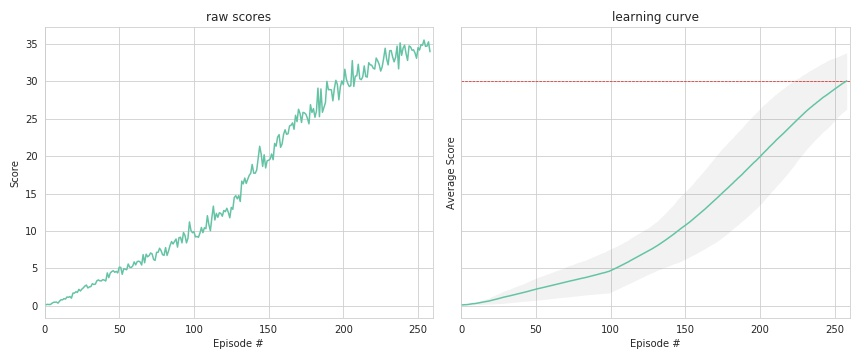
\includegraphics[width=0.60\textwidth]{../notebooks/figures/2018-10-22-PPO-learning-curve.jpg}
\caption{PPO with actor/critic - Learning Curve(left panel) and Moving-average(right panel)}
\label{fig:ppo}
\end{figure}


I used the same network configurations of the DDPG. I used a replay buffer size of $100,000$ experiences, mini-batches of $62$ instances and a discount factor of $0.99$. I used $\epsilon=0.1$ to clip the surrogate function and $\beta=0.1$ to modulate the entropy bonus. Both variables vanished over time, as in Udacity implementation. I also used $\tau=0.95$ as the GAE lambda factor used in the advantage estimator. Finally, I optimized the surrogate loss four times on each mini-batch. This model was able to solve the environment in $258$ episodes. The figure \ref{fig:ppo} presents the results of the simulation.


 % The submission reports the number of episodes needed to solve the environment.
The table \ref{tab:final_results} below presents the final performance of each algorithm tested. The error margins were computed using the standard deviation of the distribution of the final score over the last $100$ episodes. The figure \ref{fig:final_comp} presents a comparison of the moving average of $100$ episodes of the scores achieved by each model.


\begin{table}[ht!]
\centering
\begin{tabular}{lrrr}
{model} &  episodes &  Score \\
\midrule
PPO with future rewards &      3999 &    $5.58\pm0.54$ \\
PPO with actor/critic   &       258 &   $30.08\pm3.74$ \\
DDPG                    &       309 &   $30.06\pm2.52$ \\

\end{tabular}
\caption{\label{tab:final_results}Summary of the tests}
\end{table}


% plot of rewards per episode is included to illustrate that either: [version 2] the agent is able to receive an average reward (over 100 episodes, and over all 20 agents) of at least +30

\begin{figure}[ht]
\centering
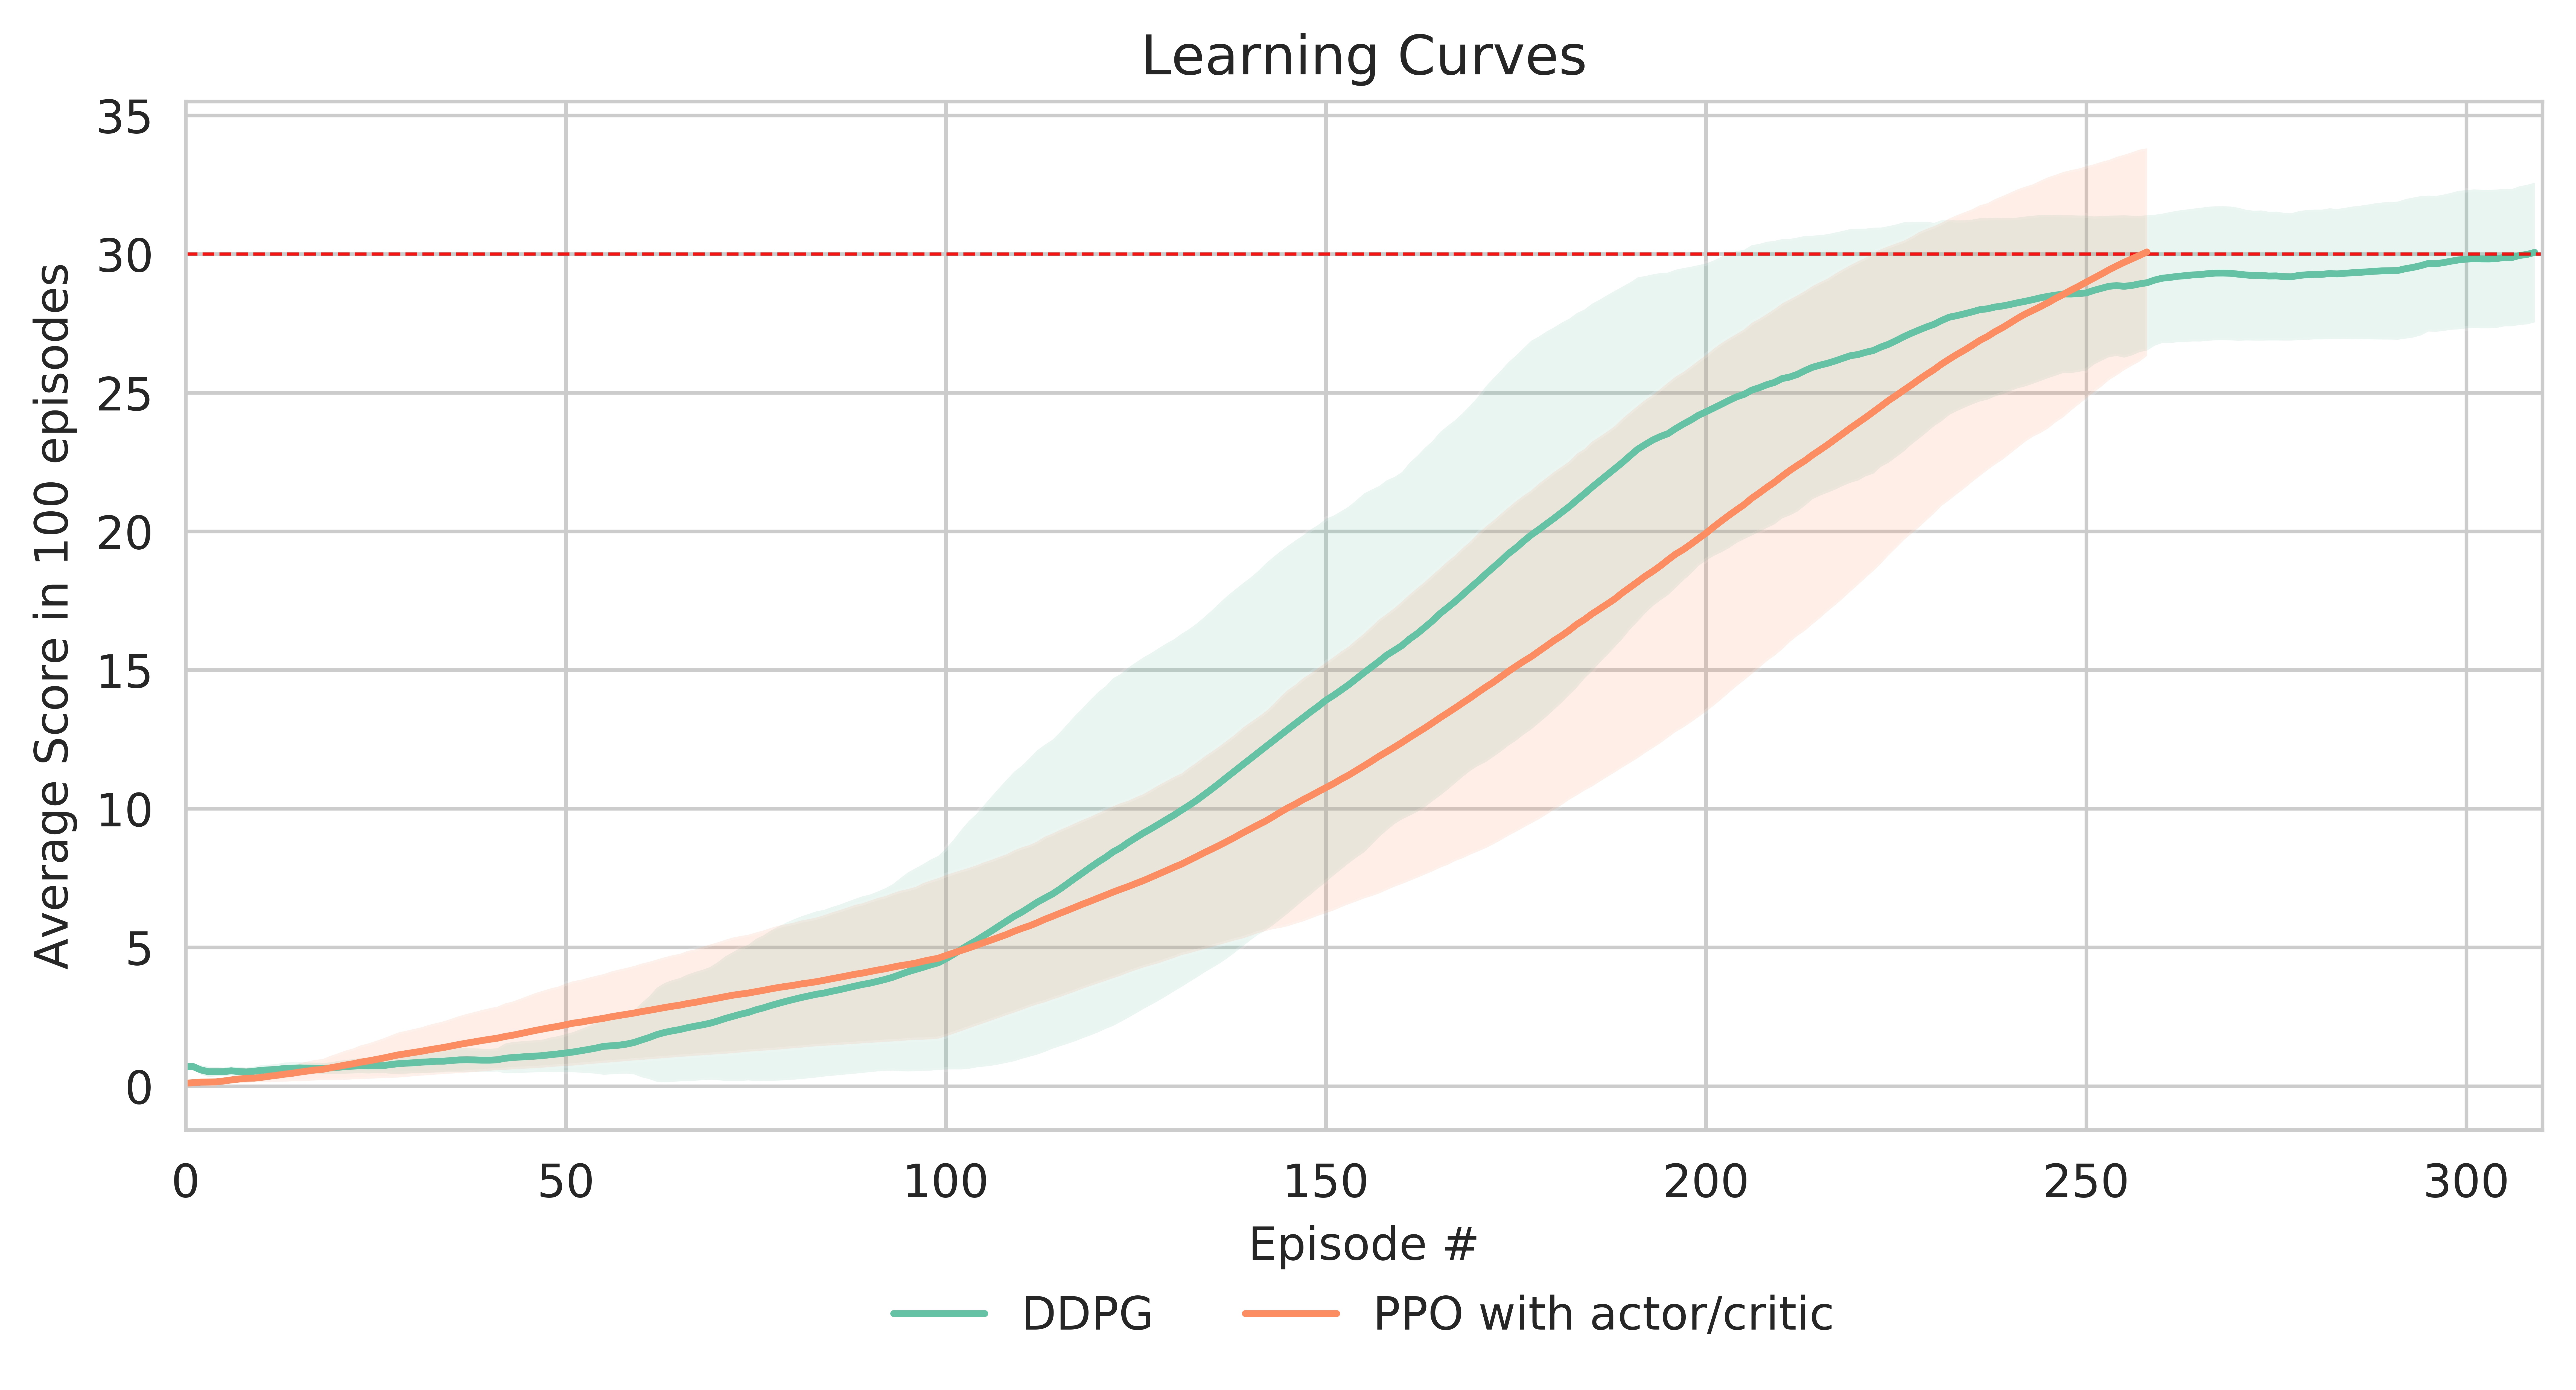
\includegraphics[width=0.65\textwidth]{../notebooks/figures/2018-10-22-final-comparition.jpg}
\caption{Moving Average of $100$ episodes of the score}
\label{fig:final_comp}
\end{figure}


% The submission has concrete future ideas for improving the agent's performance.
Finally, as some possibles extensions, the parameters of the models could be better tuned, and another model could be added to the analysis, as the Trust Region Policy Optimization (TRPO), presented by \cite{Schulman:2015uk}. As suggested by \cite{Duan:2016ur}, this algorithm constrains the change in the policy distribution, resulting in more stable learning in continuous control environments.




% ----------------end of document body---------------------

%---------------- start of references------------------

\bibliographystyle{plain}
% or try abbrvnat or unsrtnat
\bibliography{biblio.bib}

%---------------- end of references------------------


\end{document}
